\chapter{The role of Software in Scientific investigation}
\label{ch:Roles}

%
% Section: Intro

Nowadays scientific research is unthinkable without a use of software and investigations in various areas of science are becoming increasingly reliant on software tools \citep{goble2014better, storer2017bridging, hannay2009scientists, jimenez2017four}. \\

A software is very important asset for building a scientific knowledge and more discoveries in a research are made possible than ever by a use of software tools that automate processing of huge amount of data \citep{jimenez2017four}. Typically a software is used in a research for data processing tasks such as data analysis, modeling, simulation, control processes, knowledge dissemination, etc. \citep{hannay2009scientists, pan2016disciplinary}. \\



In modern research, a scientific software is as important as any lab-equipment \citep{wilson2014best}. However, the development of scientific software is much more complicated and fundamentally different from an ordinary commercial software like accounting software. Scientific software requires specialized domain knowledge for its development and requires a direct involvement of domain expert or scientist \citep{wilson2014best, segal2008developing}. Due to this, an increasing number of scientists are developing a software as part of their research work or directly taking part in the development process of a research software \citep{jimenez2017four, kanewala2014testing}. \\

Scientific software is a subset of software which is often times developed by a researcher being part of a research work. In a broader sense, any software can also be regarded as scientific software as long as at least one researcher uses it for a research \citep{VanessaResearch2020}. However, scientific software in this work specifically refers to software tools which are typically used in formal research and scientific activities such as hypothesis testing, simulation, mathematical modeling, etc.  \\

According to surveys conducted in the \ac{UK} and \ac{USA}, 2008 and 2017 respectively, most scientists agree that software plays an important role in their research work \citep{hettrick2014uk, nangia2017track}. Participants of the survey, in \ac{UK}, were 2000 researchers working in various areas of science in roles ranging from student to senior academic staff whereas participants of the survey, in \ac{USA}, were members of the US National Postdoctoral Association. \\
 
\noindent The results from of \ac{UK} survey indicate that \citep{hettrick2014uk}:
\begin{itemize}%[noitemsep,topsep=5pt, leftmargin=0.3in] % decrease the space between bullets
	\itemsep0em 
	\item 38\% of researchers spend at least 20\% of their time developing a software.
	\item Almost half of scientists spend more time creating software as part of their research work than five years ago .
	\item Over 50\% of survey respondents reported that they develop their own software. 
	\item Nearly 70\% claim their research-work directly depends on use of a software and
	\item Over 90\% of scientists say software is important for their research. \\
\end{itemize}

\noindent The results from of \ac{USA} survey indicate that \citep{nangia2017track}:
\begin{itemize}%[noitemsep,topsep=5pt, leftmargin=0.3in] % decrease the space between bullets
	\itemsep0em
	\item Over 90\% of scientists use software 
	\item 63\% of respondents said their research is impossible with out the use of software.
	\item 31\% of scientists stated they could do their work without using a software but more effort would require.
	\item Only 6\% of survey respondents say that there is would be no significant difference in their task if they do not have to use software. 
	
\end{itemize}

Overall, results from the two surveys clearly indicate that software is pervasive in scientific investigations and many researchers use as well as develop a software for their research. \\

Even though software plays an important role in a modern research, usually the contributions of software is understated. This can be seen from the poor citation practice of software in research papers across several fields of research \citep{schindler2021somesci,yang2018important, pan2016disciplinary}.  In attempt to promote the recognition of the roles of scientific software in a research, the \ac{ReSA} \footnote{\url{https://www.researchsoft.org/}} has collected literature that evident the roles software play in a research, at Zetoro group library \footnote{\url{https://www.zotero.org/groups/2400609/resa/library}}. The main aim of \ac{ReSA} is to influences decision makers to acknowledge contributions of a research software and give credits to its developers.\\

The next section presents more details about the role of software: in general, in specific domains, and in research breakthroughs.


%-----------------------------
\section{General roles}
%-----------------------------
\label{sec:Roles:Generalroles}

Software is playing crucial roles in a research and making a shift in a research culture in terms of  enabling automation of analysis pipelines, creation of new ways of analysis via computational models, supporting sophisticated analysis of large volume of data, documentation of a research, etc. \citep{jay2020software}. \\

\noindent Some of the most general roles of a software in research are:

\begin{itemize}%[noitemsep,topsep=5pt, leftmargin=0.5in] % decrease the space between bullets
	\itemsep0em
	\item A software dictates the quality of a research outcome \citep{hannay2009scientists}. Outcome of a research becomes unreliable or even useless if there is an error in the software \citep{soergel2014rampant}. For example, several scientists retracted their scientific publications up on a retrospective discovery of a bug in their software \citep{wilson2014best,merali2010computational,miller2006scientist}. A more palpable failure of a research ambition due to an error in the software, for instance, is the failure of Ariane rocket in 1996 \citep{enwiki:1054482061}.  
	\item Software helps to explore and understand a research problem \citep{hannay2009scientists}.
	\item Results from a scientific software is presented as an evidence to support a research conclusion \citep{kanewala2014testing}. 
	
  
	
	\item A software also helps to document a research process and to validate results of a given research \citep{jay2020software}. Executable cells in a Jupyter notebook is one real world example where a software can be used to validate a research result.
	
	\item Software allows experiments to be made beyond constrains of the physical world. This is because experiments that run on a computer are not limited by processes that occur in nature but only by the laws embedded in the computer code \citep{wolfram1984computer}. 

\end{itemize}

%-----------------------------
\section{Domain Specific Examples}
%-----------------------------
\label{sec:Roles:Domain}

A software is being extensively used for a research in various areas of science such as physics, chemistry, space science, life science and so on.\\

The physics research facility, the \ac{LHC} at \ac{CERN}, for instance uses a software with more than 5 million lines of code which is used for processing of terabytes of data generated from experiments \citep{storer2017bridging}.\\

In a nuclear research, a software is being developed increasingly to be used for experiments \citep{yan2017case}. For example, testing a modification in a nuclear weapon can not be done on a field, but instead a software that simulate the impact of modification is usually used \citep{kanewala2014testing}. This is because testing of a nuclear weapon on a field is banned by regulations like nuclear test ban treaties \ac{NTBT} in addition to the potential disaster that testing a nuclear weapon poses to the environment and life \citep{enwiki:1053274189}. \ac{Geant4} is example of software tool that is typically used in nuclear research to simulate the passage of particles through a matter \citep{enwiki:1077695266}.  \\


In chemistry research, a software can be used to model and simulate chemical processes that are challenging, too complex or expensive to conduct in reality. Karplus and Levitt used computer simulations for their joint-research “the development of multi-scale models for complex chemical systems”  and won a Nobel prize in 2013 for their work \citep{storer2017bridging, andre2014nobel}.\\

In a climate and environmental studies, software is used to make predictions about climate changes. For example historical temperature data can be integrated to make predictions about future temperature variations \citep{storer2017bridging}.  \\


In a space science, space probes heavily rely on software. In this case a software navigates space crafts to other planets, processes and transmits scientific data back to Earth for further processing, helps researchers interpret results, etc.\citep{lutz2011software}. CODE-A is one example of software framework used by \ac{NASA} to transmit observation information securely to a remote computer systems \citep{NASA2022}. \\

In medical research and diagnosis, imaging software plays a critical role to assist medical researchers, for instance, for early isolation of cancer cells.  The main reason for low chance of survival from cancer is mainly due to late detection of cancer cells in the body. This makes a diagnosis of cancer to be a time critical task and early identification of cancer implies curability of a disease and a higher chance of survival \citep{wagner2004challenges}. Especially on the early stages, it is not straight forward to determine which cells are likely to develop a cancer. For this reason, medical scientists use different types of software to identify cancer cell or to decide weather a tumor is malignant or not. Using a software, they could perform various kinds of analysis and processing on imageries obtained from scans such as \ac{MRI} or \ac{CT} Scan \citep{al2012lung}. An example of software that is used for cancer imaging research is \ac{DMRI}. Such software is extensively used by many researchers, more than 75,000 downloads every year \citep{norton2017slicerdmri}. Therefore, it is clear that software plays a critical role in medicine, to diagnose diseases and ultimately to save life. \\


Software plays an important role in power system planning and operation as well. One of the major activities in power system operation is contingency analysis. During contingency analysis, engineers determine violations of power grid operation conditions, such as overloading, which might occur when outage of a transmission line or a power generation unit happens. Contingency analysis helps to understand power system behavior after outages and gives an opportunity to take preventative actions \citep{mishra2012contingency}. Power grids are extremely complex and such kind of analysis tasks are unimaginable with out a use of software. An example of software that is used to perform contingency analysis in the power system operation is \emph{Power World} software  \footnote{\url{https://www.powerworld.com/}}. \\

Though it is not possible to mention the role and use of software across all areas of science and research, the above examples serve to be a good sample to see how ubiquitous the impact of software is  almost in all research areas. 


%
% Section:The Role in Research Breakthroughs

%-----------------------------
\section{The role of software in research breakthroughs }
%-----------------------------
\label{sec:Roles:breakthroughs}

The impact of software is more pronounced and easy to observe when scientists achieve ground breaking results. The use of software enabled scientists to produce better scientific discoveries and achieve research breakthroughs \citep{goble2014better}. \\

One good example of research breakthrough made, because of use of software in a scientific investigation,  is creation of the very first visual representation of a black hole using an open source software  NumFOCUS\footnote{\url{https://numfocus.org/}} \citep{event2019first}. \\

To observe a black hole that is 55 million light years away, it would have required to build a huge telescope of size of planet earth. But instead of building one giant telescope, which is not possible any way, hundreds of scientists spent decades of years creating a global network of telescopes, known as  \ac{EHT} \citep{enwiki:1052167868}, synchronized precisely using atomic clocks. \\

\begin{figure}[htbp]
	\centering
	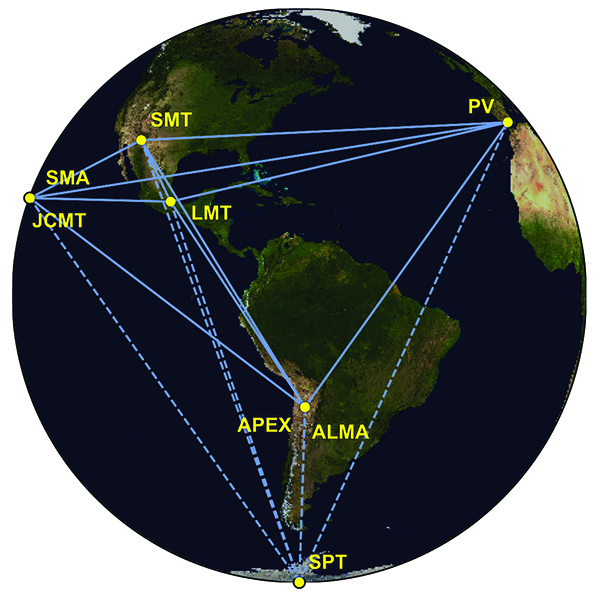
\includegraphics[width=.45\textwidth]{4.graphics/figures/ch_2/EHT}
	\caption{Location of \ac{EHT} Satellites around the world}
	\label{fig:chapter03:setup}
\end{figure}

The \ac{EHT} gathered a huge amount of data for years. However there was a lot of noise in the collected data because the \ac{EHT} was a network  non-similar telescopes. In addition, the radio signals were coming through attenuated due to atmospheric effects like water vapor, clouds, turbulence, etc. \citep{NumFOCUSblackhole}.\\

Therefore the scientists had to use various algorithms and data analysis pipelines. The resulting image from various data processing was compared to ensure the integrity of the result. This huge scientific breakthrough in a space research, can be attributed to the use of powerful data processing software. 






